\section{Graded Assignment 1}\label{sec:graded_assignment_1}

\begin{figure}[ht]
	\begin{subfigure}[b]{0.4\textwidth}
		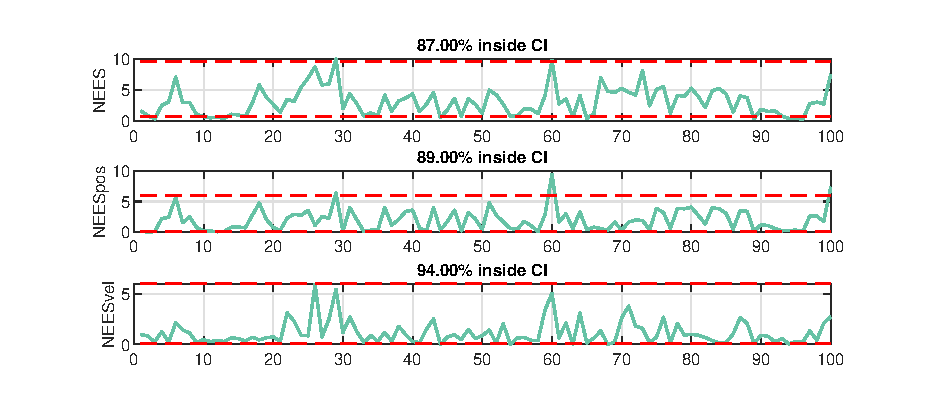
\includegraphics[width=\textwidth]{figures/ga_1/2_NEES}
		\caption{}
		\label{fig:ga_1_2_NEES}
	\end{subfigure}%
       ~
	\begin{subfigure}[b]{0.4\textwidth}
		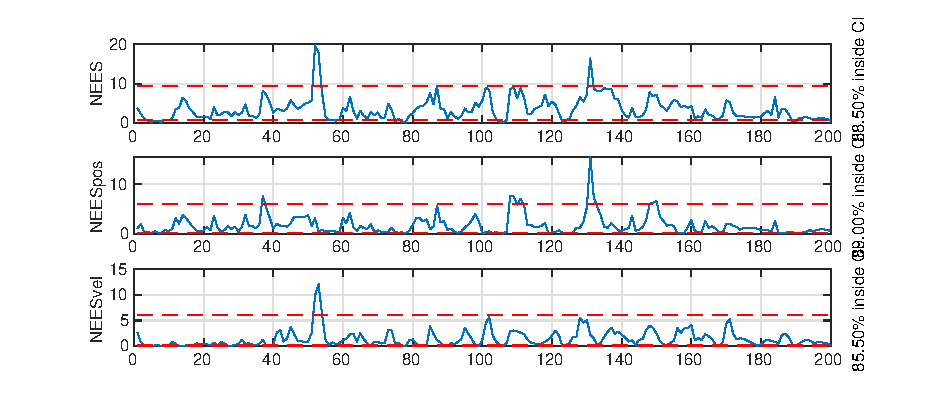
\includegraphics[width=\textwidth]{figures/ga_1/joyride_NEES}
		\caption{}
		\label{fig:ga_1_joyride_NEES}
	\end{subfigure}
        \\
    \begin{subfigure}[b]{0.4\textwidth}
        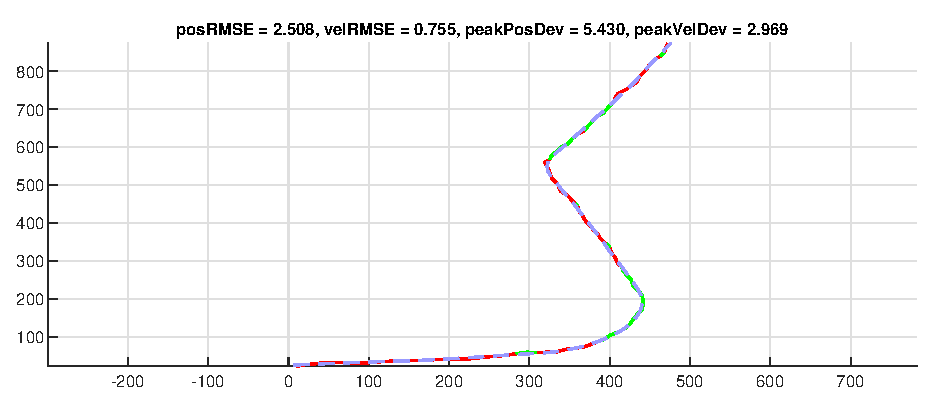
\includegraphics[width=\textwidth]{figures/ga_1/2_estimated_trajectory}
        \caption{}
        \label{fig:ga_1_2_estimated_trajectory}
    \end{subfigure}%
        ~
    \begin{subfigure}[b]{0.4\textwidth}
        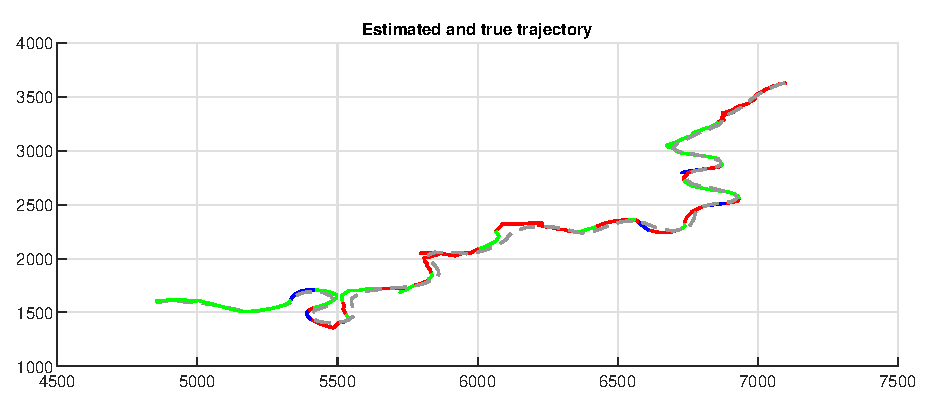
\includegraphics[width=\textwidth]{figures/ga_1/joyride_estimated_trajectory}
        \caption{}
        \label{fig:ga_1_joyride_estimated_trajectory}
    \end{subfigure}
        \\
    \begin{subfigure}[b]{0.4\textwidth}
        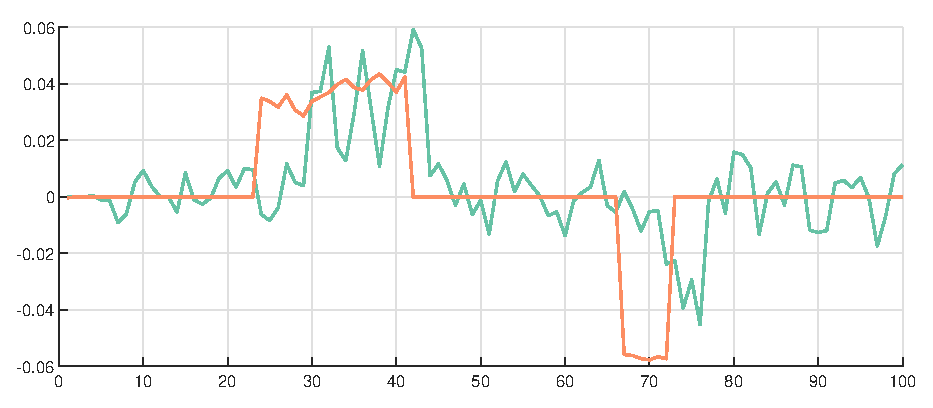
\includegraphics[width=\textwidth]{figures/ga_1/2_error}
        \caption{}
        \label{fig:ga_1_2_error}
    \end{subfigure}%
        ~
    \begin{subfigure}[b]{0.4\textwidth}
        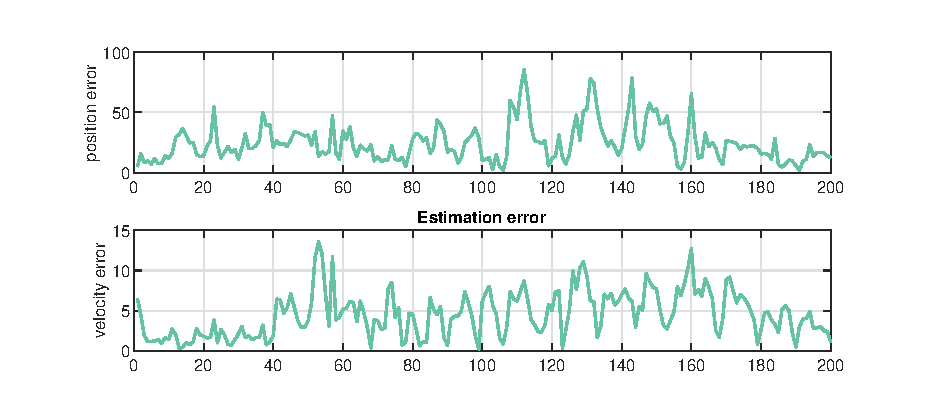
\includegraphics[width=\textwidth]{figures/ga_1/joyride_error}
        \caption{}
        \label{fig:ga_1_joyride_error}
    \end{subfigure}
    \label{fig:ga_1} 
\end{figure}

% task 2 and 3
    % NEES with confidence bounds
        % total
        % position
        % velocity
    % estimation error (Euclidian distance)
        % position 
        % velocity
    % averaged NEESes 
    % number of times the NEESes fall within the confidence region
    % position and velocity RMSE (mean taken over time)

% parameters based on this
% other plots




% For task 2 and 3, we want to see a plot of the total, position and velocity NEES along with your chosen confidence bounds for these, and estimation error (Euclidian distance) in position and velocity for the tracker run with your chosen parameters. 
% In addition we want the numbers of the averaged NEESes along with their confidence bounds, the number of times the NEESes fall within the confidence regions and the positional and velocity RMSE (mean taken over time). 
% We then expect you to base your choice of parameters on these values, and compare to other sets of parameters. 
% To show plots of other parameter settings is up to you. 